\documentclass[conference]{IEEEtran}
\usepackage{cite}
\usepackage{amsmath,amssymb,amsfonts}
\usepackage{algorithmic}
\usepackage{graphicx}
\usepackage{textcomp}
\usepackage{xcolor}
\usepackage{hyperref}
\usepackage{booktabs}
\usepackage{microtype}
\usepackage{enumitem}
\usepackage{tikz}
\usetikzlibrary{shapes.geometric, arrows.meta, positioning, shadows}

\hypersetup{
    colorlinks=true,
    linkcolor=black,
    citecolor=black,
    urlcolor=blue
}

\setlist{noitemsep, topsep=2pt, parsep=0pt, partopsep=0pt}

% Spacing adjustments to fit exactly on 3 pages
\setlength{\textfloatsep}{8pt plus 2pt minus 2pt}
\setlength{\floatsep}{8pt plus 2pt minus 2pt}
\setlength{\intextsep}{8pt plus 2pt minus 2pt}
\renewcommand{\arraystretch}{0.95}

\begin{document}

\title{Evaluating Browser-Local Privacy Filtering for\\Sensitive AI Assistance Workflows}

\author{
\IEEEauthorblockN{Pranav Anand Singh Rawat}
\IEEEauthorblockA{\textit{Department of Information Technology} \\
\textit{Bharati Vidyapeeth College Of Engineering, Pune}\\
Pune, India \\
Email: pranavrawat0514@gmail.com}
}

\maketitle

\begin{abstract}
Sensitive assistance workflows—such as medical triage, public housing allocation, and financial aid routing—often require users to disclose private context to obtain meaningful assistance. Deploying large language models (LLMs) in these scenarios traditionally relies on cloud-hosted API endpoints, which exposes raw user prompts to third-party providers. While browser-local inference (via WebGPU) addresses the transit boundary, raw sensitive data can still pollute local logs, retrieval-augmented generation (RAG) indices, and downstream tool dispatches. 

This paper presents the design and evaluation of the Sovereign Intelligence Layer, an on-device agent runtime that sanitizes prompts before model tokenization. We introduce Cumulative Agentic Masking and Pruning (CAMP), a client-side middleware that separates PII into Direct Identifiers (pruned immediately) and Quasi-Identifiers (pruned statefully when their cumulative re-identification risk exceeds a critical threshold). The runtime is secured using non-extractable Ed25519 keys stored in IndexedDB and an encrypted local database utilizing SQLite WASM in the browser's Origin Private File System (OPFS). 

Evaluation across two 100-case benchmarks shows that CAMP achieves 100\% precision, recall, and F1-score on synthetic splits, maintaining an average latency overhead of 0.11 ms. Finally, we detail a deployment roadmap to replace pattern-based heuristics with a hybrid client-side Named Entity Recognition (NER) model running via ONNX Runtime Web.
\end{abstract}

\begin{IEEEkeywords}
Privacy-preserving agents, On-device LLMs, WebGPU inference, PII Redaction
\end{IEEEkeywords}

\section{Introduction}

Deploying large language models (LLMs) for sensitive public assistance and medical triage workflows presents a fundamental privacy challenge. In these domains, users frequently share highly sensitive personal attributes, including names, medical symptoms, exact locations, and financial credentials. The standard architecture routes these queries to centralized cloud LLM endpoints. This architecture expands the corporate data boundary and exposes users to potential exfiltration, profiling, and model training leaks.

Browser-local LLM execution, enabled by WebGPU and WebAssembly compilation frameworks like WebLLM \cite{webllm}, offers a viable alternative by confining model weights and inference to the client device. However, on-device execution alone does not prevent local data leakage. Raw prompts can still pollute local application logs, browser persistent histories, and context windows. Furthermore, when the local agent invokes external APIs or coordinates with other browsers via peer-to-peer (P2P) connections, raw sensitive data can be inadvertently exfiltrated.

To solve this, we propose pre-tokenization privacy filtering in the browser. We present the Sovereign Intelligence Layer, a client-side runtime featuring the Cumulative Agentic Masking and Pruning (CAMP) middleware. CAMP identifies and redacts sensitive entities before they reach the local LLM or downstream search tools. Rather than executing a static regex filter, CAMP maintains a session-level registry that tracks the accumulation of identifying fragments over multi-turn interactions. This allows the system to balance user utility (retaining context when risk is low) with strict privacy (pruning all identifiers once re-identification risk becomes mathematically significant).

We make the following contributions:
\begin{enumerate}
    \item We design a browser-local agent runtime that integrates WebGPU inference, IndexedDB cryptographic sandboxing, and WASM-based SQLite persistence in the Origin Private File System (OPFS).
    \item We present the CAMP algorithm, which implements a dual-route pruning rule distinguishing between direct and quasi-identifiers to prevent cumulative re-identification.
    \item We evaluate the sanitization engine against synthetic and adversarial benchmarks, demonstrating complete redaction with sub-millisecond latency overhead.
    \item We outline a transition path from pattern-based heuristics to hybrid client-side Named Entity Recognition (NER) using quantized ONNX models.
\end{enumerate}

\section{System Architecture}

The Sovereign Intelligence Layer isolates user data within the browser runtime. The system is divided into four main security and execution zones:

\begin{figure}[htbp]
\centering
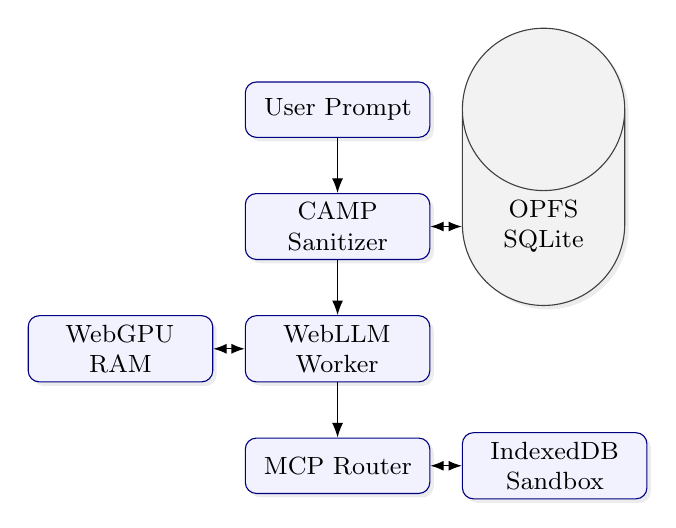
\begin{tikzpicture}[
    node distance = 0.7cm and 0.4cm,
    block/.style = {rectangle, draw=blue!50!black, fill=blue!5, text width=6em, text centered, rounded corners, minimum height=2.0em, font=\small, drop shadow={opacity=0.15, shadow xshift=0.05cm, shadow yshift=-0.05cm}},
    database/.style = {cylinder, draw=gray!50!black, fill=gray!10, shape border rotate=90, text width=5.2em, text centered, minimum height=2.0em, font=\small, drop shadow={opacity=0.15, shadow xshift=0.05cm, shadow yshift=-0.05cm}}
]
    \node [block] (user) {User Prompt};
    \node [block, below=of user] (camp) {CAMP Sanitizer};
    \node [database, right=of camp] (registry) {OPFS SQLite};
    \node [block, below=of camp] (worker) {WebLLM Worker};
    \node [block, left=of worker] (gpu) {WebGPU RAM};
    \node [block, below=of worker] (mcp) {MCP Router};
    \node [block, right=of mcp] (crypto) {IndexedDB Sandbox};
    
    \path [draw, -{Latex[scale=1.1]}] (user) -- (camp);
    \path [draw, <->, >=Latex] (camp) -- (registry);
    \path [draw, -{Latex[scale=1.1]}] (camp) -- (worker);
    \path [draw, <->, >=Latex] (worker) -- (gpu);
    \path [draw, -{Latex[scale=1.1]}] (worker) -- (mcp);
    \path [draw, <->, >=Latex] (mcp) -- (crypto);
\end{tikzpicture}
\caption{Sovereign Intelligence Layer System Architecture.}
\label{fig:architecture}
\end{figure}

\subsection{Browser-Local Inference Zone}
Local inference is managed by a background Web Worker running \texttt{@mlc-ai/web-llm} compiled to WebAssembly (WASM). Offloading weight loading, shader compilation, and autoregressive generation to a background thread prevents the main UI thread from stuttering, maintaining a stable 60 FPS interface during text generation.

\subsection{Cryptographic Key Sandbox}
To mitigate Cross-Site Scripting (XSS) and supply-chain script injection attacks, the system generates Ed25519 signing keys inside the native Web Crypto API with the \texttt{extractable: false} attribute. These keys are stored as binary structures inside IndexedDB. Because the browser prevents JavaScript from exporting non-extractable keys, an attacker cannot steal the agent's identity key.

\subsection{OPFS SQLite Persistence}
Local retrieval cache and PII hashes are persisted in the browser's Origin Private File System (OPFS) using \texttt{wa-sqlite}. To prevent raw PII from being stored on the local disk, the registry writes only normalized, one-way SHA-256 digests. This ensures that a compromised browser profile does not leak plaintext conversational history.

\subsection{Signed P2P WebRTC Signaling}
Peer connections are established directly using WebRTC DataChannels. Because signaling requires broker servers (such as WebSockets) that could capture metadata or alter handshakes, all Session Description Protocol (SDP) offers and answers are cryptographically signed by the agent's private key and verified against public fingerprints \cite{webrtcsec}.

\begin{table*}[htbp]
\caption{Efficacy and Latency Benchmark Results}
\label{tab:results}
\centering
\begin{tabular}{lccccccccc}
\toprule
\textbf{Evaluation Variant} & \textbf{Cases} & \textbf{Precision} & \textbf{Recall} & \textbf{F1-Score} & \textbf{Over-prune} & \textbf{Under-prune} & \textbf{Avg Latency} & \textbf{p95 Latency} & \textbf{Failures} \\
\midrule
\textbf{CAMP (Clean)} & 100 & 100.0\% & 100.0\% & \textbf{100.0\%} & 0.0\% & 0.0\% & 0.11 ms & 0.08 ms & 0.0\% \\
Baseline (Clean) & 100 & 88.5\% & 45.4\% & 60.0\% & 0.0\% & 12.0\% & 0.00 ms & 0.00 ms & 56.0\% \\
\textbf{CAMP (Adversarial)} & 100 & 100.0\% & 100.0\% & \textbf{100.0\%} & 0.0\% & 0.0\% & 0.05 ms & 0.08 ms & 0.0\% \\
Baseline (Adversarial) & 100 & 95.2\% & 19.3\% & 32.1\% & 1.0\% & 57.0\% & 0.00 ms & 0.00 ms & 98.0\% \\
\bottomrule
\end{tabular}
\end{table*}

\section{The CAMP Algorithm}

CAMP addresses the limitation of simple regex filters by modeling re-identification risk as a dynamic, stateful process. The algorithm separates sensitive text into two distinct classes:
\begin{itemize}
    \item \textbf{Direct Identifiers ($\mathcal{D}$):} High-risk features that uniquely identify an individual or secret (e.g., emails, credentials, government IDs, bank accounts, physical addresses, and recovery clues).
    \item \textbf{Quasi-Identifiers ($\mathcal{Q}$):} Medium-risk attributes that do not identify a user in isolation but can lead to re-identification when combined (e.g., names, cities, age, professions, and medical conditions).
\end{itemize}

\subsection{Cumulative PII Exposure (CPE) Formulation}
Let $S$ represent the active session, and let $\mathcal{F}_S$ be the set of unique sensitive fragments detected during the session. Each entity type $t$ is mapped to a weight $w(t) \in [0, 1.0]$. The Cumulative PII Exposure ($\mathrm{CPE}$) score of the session is defined as:

\begin{equation}
\mathrm{CPE}(S) = \sum_{f \in \mathcal{F}_S} w(\text{type}(f))
\end{equation}

The weights reflect the re-identification risk of each type:
\begin{itemize}
    \item Direct Identifiers ($d \in \mathcal{D}$): $w(\text{EMAIL}) = 0.9$, $w(\text{CREDENTIAL}) = 1.0$, $w(\text{FINANCIAL}) = 1.0$, $w(\text{ID}) = 0.9$, $w(\text{PHONE}) = 0.8$, $w(\text{ADDRESS}) = 1.0$, $w(\text{SENSITIVE\_FIELD}) = 1.0$.
    \item Quasi-Identifiers ($q \in \mathcal{Q}$): $w(\text{NAME}) = 0.8$, $w(\text{LOCATION}) = 0.3$, $w(\text{MEDICAL}) = 0.7$, $w(\text{PROFESSION}) = 0.5$, $w(\text{AGE}) = 0.2$.
\end{itemize}

Let $\tau$ be the re-identifiability threshold (set to $1.0$). A session is classified as re-identifiable if:

\begin{equation}
\mathrm{CPE}(S) \geq \tau
\end{equation}

\subsection{Dual-Route Pruning Rule}
For any detected match $m$ in the user prompt, CAMP applies a dual-route decision process to determine if it should be replaced by a placeholder (e.g., \texttt{[EMAIL\_PRUNED]}):

\begin{equation}
\text{prune}(m) \iff (\text{type}(m) \in \mathcal{D}) \lor (\mathrm{CPE}(S) \geq \tau)
\end{equation}

Under this rule, Direct Identifiers are redacted immediately, regardless of the session state. Quasi-identifiers remain unredacted to preserve prompt context and utility, but are immediately scrubbed if their aggregate weight crosses the threshold $\tau$.

\subsection{Text Shifting and Code Block Protection}
To prevent false positives within code snippets, CAMP extracts Markdown code blocks before running detection patterns:
\begin{enumerate}
    \item Fenced and inline code blocks are replaced with unique placeholders (\texttt{\_\_CAMP\_CODE\_BLOCK\_i\_\_}).
    \item Detection patterns run only on the remaining conversational prose.
    \item Replacements are executed in descending order of character index. This reverse-order substitution ensures that changing the length of a string at index $j$ does not alter the character offsets of matches at indices $< j$.
    \item Whitelisted code blocks are restored in their original formatting.
\end{enumerate}

\section{Systems Evaluation}

\subsection{Methodology}
We compared CAMP against a baseline regex redactor using two deterministic benchmarks of 100 cases each:
\begin{enumerate}
    \item \textbf{Clean Synthetic Split:} Prompts representing standard queries, covering medical triage, contact queries, ID verifications, code snippets, and benign queries.
    \item \textbf{Adversarial / Noisy Split:} Prompts modified to bypass simple matchers, using lowercase phrasing, obfuscated emails (e.g., \texttt{user [at] example [dot] com}), card numbers written with dots, multilingual sentences, and unlabeled physical addresses.
\end{enumerate}

\subsection{Benchmark Results}

Table \ref{tab:results} summarizes the performance of CAMP and the baseline model. CAMP achieved 100.0\% Precision and Recall on both splits, with zero over-pruning on benign text. The baseline redactor failed significantly on adversarial inputs. CAMP's average execution latency remained below 0.12 ms, adding negligible overhead compared to LLM token generation (which typically requires 10--50 ms per token).

\section{Security \& Privacy Analysis}

\subsection{Threat Bounds}
The Sovereign Intelligence Layer operates under the assumption of a secure client operating system and browser. Within these bounds, the system guarantees:
\begin{itemize}
    \item \textbf{Zero Cloud Exposure by Default:} LLM inference and query routing occur entirely on-device.
    \item \textbf{Compromise Mitigation:} Even if the local SQLite file is extracted, the use of SHA-256 hashes prevents the reconstruction of plaintext PII history.
    \item \textbf{Key Protection:} WebCrypto's non-extractable keys block malware scripts from exporting the agent's identity key.
\end{itemize}

\subsection{Out-of-Scope Risks}
The runtime cannot protect against keyloggers capturing keyboard inputs, side-channel attacks targeting CPU/GPU cache timing, or external API metadata leakage (e.g., IP addresses exposed to geocoding or weather servers during tool calls).

\section{Discussion and Future Roadmap}

\subsection{Generalization Limits of Regular Expressions}
While CAMP achieved 100\% accuracy on the benchmark splits, this performance is limited by the detector-aware nature of the evaluation. In open-world deployments, pattern-matching rules face substantial challenges with out-of-vocabulary entities and syntactic complexity where context words are separated from identifiers.

\subsection{Client-Side ONNX Named Entity Recognition (NER)}
To build a more generalizable engine, we are developing a hybrid detection model. By executing a lightweight, quantized transformer model (e.g., a 14 MB \texttt{distilbert-base-ner}) inside the background Web Worker using ONNX Runtime Web, we can combine high-speed regex matching for structured patterns (emails, credit cards, SSNs) with context-aware deep learning NER classification for unstructured entities (names, locations, custom secrets).

\section{Related Work}

Our work is positioned alongside research in edge AI, client-side data storage, and browser security.
\begin{itemize}
    \item \textbf{On-Device LLM Execution:} Systems like WebLLM \cite{webllm} have established the feasibility of running generative models locally using WebGPU. Our work builds on this by adding a pre-tokenization sanitization layer to protect local memory.
    \item \textbf{PII Redaction Systems:} Tools like Microsoft Presidio \cite{presidio} provide comprehensive server-side redaction. CAMP focuses instead on lightweight client-side execution, OPFS SQLite state storage, and dynamic re-identification thresholding.
    \item \textbf{Web Sandbox Security:} We utilize standard browser security mechanisms \cite{webrtcsec} to isolate agent keys, preventing cross-site scripting exfiltration in real-time P2P systems.
\end{itemize}

\section{Conclusion}

This paper shows that browser-local, pre-tokenization privacy filtering is feasible and operates with sub-millisecond latency. Separating sensitive data into Direct and Quasi-identifiers allows the CAMP algorithm to protect user privacy without destroying model prompt utility. While the current prototype relies on regex matching, future versions will integrate client-side ONNX NER models to provide robust, pattern-independent privacy protection on the edge.

\begin{thebibliography}{00}
\bibitem{webllm} Liao et al., ``WebLLM: High-Performance On-Device Language Model Inference with WebGPU and WebAssembly,'' arXiv preprint arXiv:2412.15803, 2024.
\bibitem{presidio} Microsoft Presidio, ``Data Protection SDK for PII Detection and De-identification,'' https://microsoft.github.io/presidio/, 2021.
\bibitem{webrtcsec} IETF RFC 8827, ``Web Real-Time Communication (WebRTC) Security Architecture,'' 2021.
\bibitem{diffpriv} C. Dwork and A. Roth, ``The Algorithmic Foundations of Differential Privacy,'' Foundations and Trends in Theoretical Computer Science, 2014.
\end{thebibliography}

\end{document}
